\begin{figure}[H]
		\begin{minipage}[t]{0.45\linewidth}
		\centering
		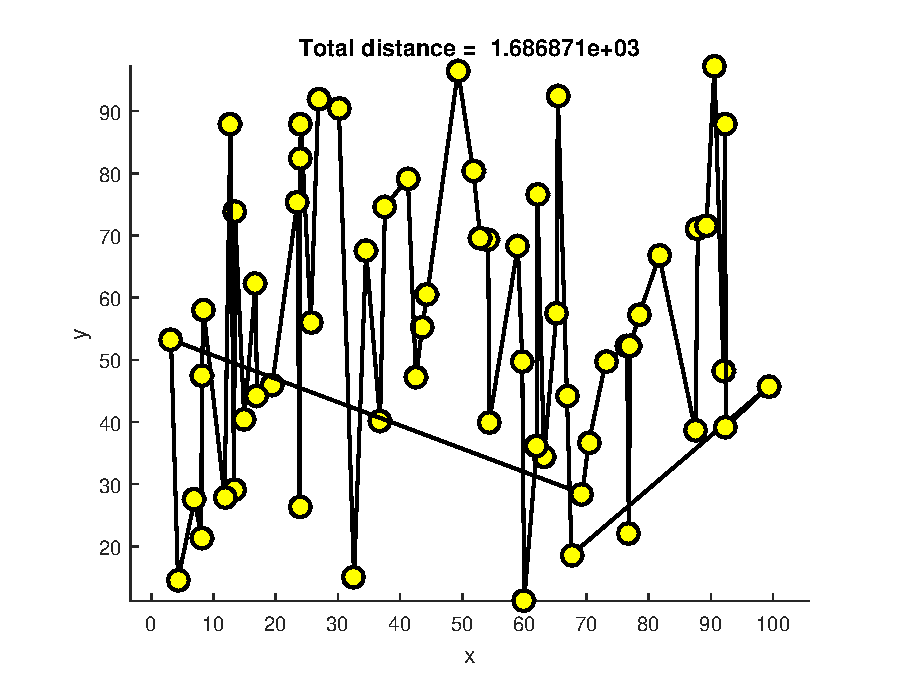
\includegraphics[width=\textwidth]{\Pathofcinq/path.eps}
		\caption{Path journey}\label{fig:Pathofcinq:path}
		
		\end{minipage}\hfill
		\begin{minipage}[t]{0.45\linewidth}
		\centering
		\includegraphics[width=\textwidth]{\Pathofcinq/AS_1_5AS_ExecTimeAndMeanSTDWith_execVariation.eps}
		\caption{Variation of the execution time VS the \# of ants (20$\stackrel{step=20}{\rightarrow}$100) in each execution (1$\stackrel{step=1}{\rightarrow}$ 5)}
		\label{fig:Pathofcinq:AS_1_5AS_ExecTimeAndMeanSTDWith_execVariation}
		\end{minipage}
	\flushleft
		\begin{minipage}[t]{0.45\linewidth}
		\centering
		\includegraphics[width=1.5\textwidth]{\Pathofcinq/AS_BestCost_Varying_Iteration_and_nbAnts.eps}
		\caption{Best cost VS Ants number variation with $\alpha$=1, $ \beta $ = 5}
		\label{fig:Pathofcinq:AS_BestCost_Varying_Iteration_and_nbAnts}
		\end{minipage}
\end{figure}
		\begin{minipage}[t]{0.9\linewidth}
		\vspace{-9mm}
		\begin{table}[H]
		\label{tab:Pathofcinq:expdeux}
		\begin{tabular}{lllll}
		\cline{1-2}
		\multicolumn{1}{|l|}{Best Costs results for experience 2}                                                           &  \multicolumn{1}{l|}{Elapsed Time, Mean, STD}                                             &  &  &  \\ \cline{1-2}
		\multicolumn{1}{|l|}{\begin{tiny}\begin{tabular}{|l|c|c|c|c|c|c|c|c|c|c|}
\hline
&\textbf{It :1}&\textbf{It :2}&\textbf{It :3}&\textbf{It :4}&\textbf{It :5}&\textbf{It :6}&\textbf{It :7}&\textbf{It :8}&\textbf{It :9}&\textbf{It :10}\\\hline
\textbf{exec :1}&678.98&678.98&678.98&673.98&673.98&673.98&673.98&673.98&670.30&670.30\\\hline
\textbf{exec :2}&700.62&687.16&686.29&686.29&686.29&656.58&656.58&656.58&656.58&656.58\\\hline
\textbf{exec :3}&680.99&644.35&644.35&644.35&644.35&644.35&644.35&644.35&644.35&644.35\\\hline
\textbf{exec :4}&677.23&665.56&665.56&665.56&665.56&665.56&632.39&632.39&632.39&632.39\\\hline
\textbf{exec :5}&683.50&683.30&650.17&650.17&650.17&614.01&614.01&614.01&614.01&614.01\\\hline
\textbf{exec :6}&643.11&643.11&635.79&635.79&635.79&635.79&635.79&635.79&635.79&635.79\\\hline
\textbf{exec :7}&632.45&632.45&632.45&630.20&630.20&609.73&609.73&609.73&609.73&609.73\\\hline
\textbf{exec :8}&634.94&634.94&618.14&618.14&618.14&618.14&618.14&618.14&618.14&618.14\\\hline
\textbf{exec :9}&646.33&645.36&627.11&617.99&617.99&617.99&617.99&617.99&617.99&617.99\\\hline
\textbf{exec :10}&647.03&638.44&638.44&630.35&615.00&615.00&615.00&615.00&615.00&615.00\\\hline
\end{tabular}
\end{tiny}} & \multicolumn{1}{l|}{\begin{tiny}\begin{tabular}{|l|c|}
\hline
&\textbf{Elapsed time}\\\hline
\textbf{exec :1}&1.74\\\hline
\textbf{exec :2}&1.74\\\hline
\textbf{exec :3}&1.72\\\hline
\textbf{exec :4}&1.73\\\hline
\textbf{exec :5}&1.73\\\hline
\textbf{exec :6}&1.74\\\hline
\textbf{exec :7}&1.73\\\hline
\textbf{exec :8}&1.72\\\hline
\textbf{exec :9}&1.71\\\hline
\textbf{exec :10}&1.72\\\hline
\textbf{ Mean}&1.73\\\hline
\textbf{ STD}&0.01\\\hline
\end{tabular}
\end{tiny} } &  &  &  \\ \cline{1-2}
																						  &                                                                     &  &  &  \\
																						  &                                                                     &  &  & 
		\end{tabular}
		\caption{Results of experience 2 on rand50.dat}
		\end{table}
		\end{minipage}